\subsection{E-step versus sleep phase}
\label{sec:estep_sleep_compare}

In this subsection, we compare the posteriors obtained by optimizing the sleep phase objective~\eqref{eq:sleep_phase_summary} 
versus optimizing the E-step objective~\eqref{eq:e_step}, also known as the ELBO. 
We demonstrate on a toy example that there exist shallow optima in ELBO where the variational posterior on locations does not concentrate around the true locations. We show that the sleep phase objective is able to avoid these shallow optima. We use simulated data with known PSF and background for this example, so the wake-phase (M-step) is not needed. 

In this toy example, we simulate a $20\times20$ single-band image, shown in Figure~\ref{fig:toy_example}. Each star has the same flux. The image is divided into four $10\times 10$ tiles, which are the inputs to the neural network. 
\begin{figure}[!h]
    \centering
    \vspace{-1em}
    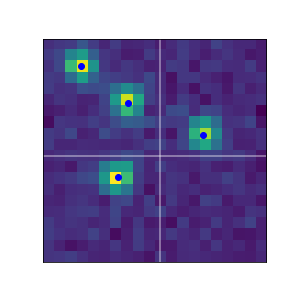
\includegraphics[width = 0.3\textwidth]{figures/vi_sleep_ex_figure.png}
    \vspace{-1.7em}
    \caption{The example $20\times 20$ image with four stars. The outlined $10\times 10$ tiles are inputs to the neural network. }
    \label{fig:toy_example}
\end{figure}

In our generative model, we set the Poisson prior parameter $\mu = 4$ and flux power law slope $\alpha = 0.5$. With these these prior parameters, optimize the ELBO and the sleep phase objective. First, in Figure~\ref{fig:optim_path} (top row), we evaluate the ELBO at the example $20\times 20$ image as the optimization proceeds. In the left-most plot, we optimized the ELBO using stochastic gradient descent with the REINFORCE estimator. The optimization did not converge, likely due to the high variance of the REINFORCE estimator. In the middle plot, we analytically integrated the ELBO with respect to the variational distribution on the number of stars $N$, and computed stochastic gradients using the reparameterization trick. See Appendix TBD for details about the gradient estimators. The stochastic gradients after integrating out $N$ exhibit lower variance, and the optimization was able to converge to stationary points. However, depending on the initialization, the variational distribution gets stuck at stationary points where the ELBO is non-optimal (e.g. restarts 3 and 6). In contrast, optimizing the sleep phase consistently converges to a similar ELBO across all restarts. 

In the bottom left of Figure~\ref{fig:optim_path}, we display the MAP locations after getting stuck in local minima in optimizing the ELBO. In the tile with two stars, both MAP locations were placed on one star. Ideally, one of the locations would be shifted to the second star. However, to move one location to the second star, the optimization path must traverse a region where the log-likelihood is lower than the current configuration. The displayed configuration is a local optima where the gradient with respect to location is approximately zero. In contrast, the sleep phase optimization consistently places MAP locations around the four true stars. An example using the first restart is shown. 

\begin{figure}[!ht]
    \centering
    \begin{subfigure}[t]{0.9\textwidth}
    \centering
    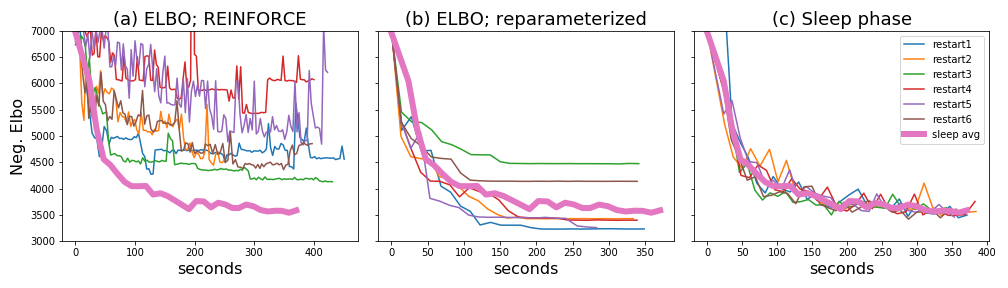
\includegraphics[width=\textwidth]{figures/optim_path_compare.png}
    \end{subfigure}
    \begin{subfigure}[t]{\textwidth}
    \centering
    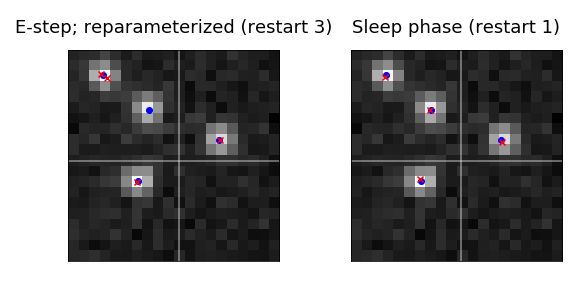
\includegraphics[width=0.55\textwidth]{figures/optim_path_detect_compare.png}
    \end{subfigure}
    \vspace{-3em}
    \caption{(Top) The ELBO as the optimization progresses, for six random restarts. Bold pink line is the sleep phase ELBO path, averaged over six restarts. (Bottom) Detections from two variational posteriors. Blue dots are true stars. Red ``x" are MAP locations under the variational posterior. }
    \label{fig:optim_path}
\end{figure}

